\documentclass[]{article}

\usepackage[a4paper, left=20mm , right=30mm , top=20mm , bottom=20mm ]{geometry}
\usepackage[ngerman]{babel}
\usepackage{hyperref}
\usepackage{capt-of}

\usepackage{amsmath}
\usepackage{amssymb}
\usepackage{bm}

\usepackage{pgfplots}
\pgfplotsset{compat=1.18}
\usepackage{circuitikz}

\usepackage[
backend=biber,
%sortlocale=de_DE,
style=numeric,
natbib=true,
url=true, 
doi=true,
eprint=false
]{biblatex}
\addbibresource{bibliography.bib}

\begin{document}
	
	\title{
		 QO100 mit Fuba DEK 417 LNB\\
		\vspace{1ex}
		\Large Dokumentation und Umbau
		\begin{minipage}{\textwidth}
			\centering
			\vspace{5ex}
			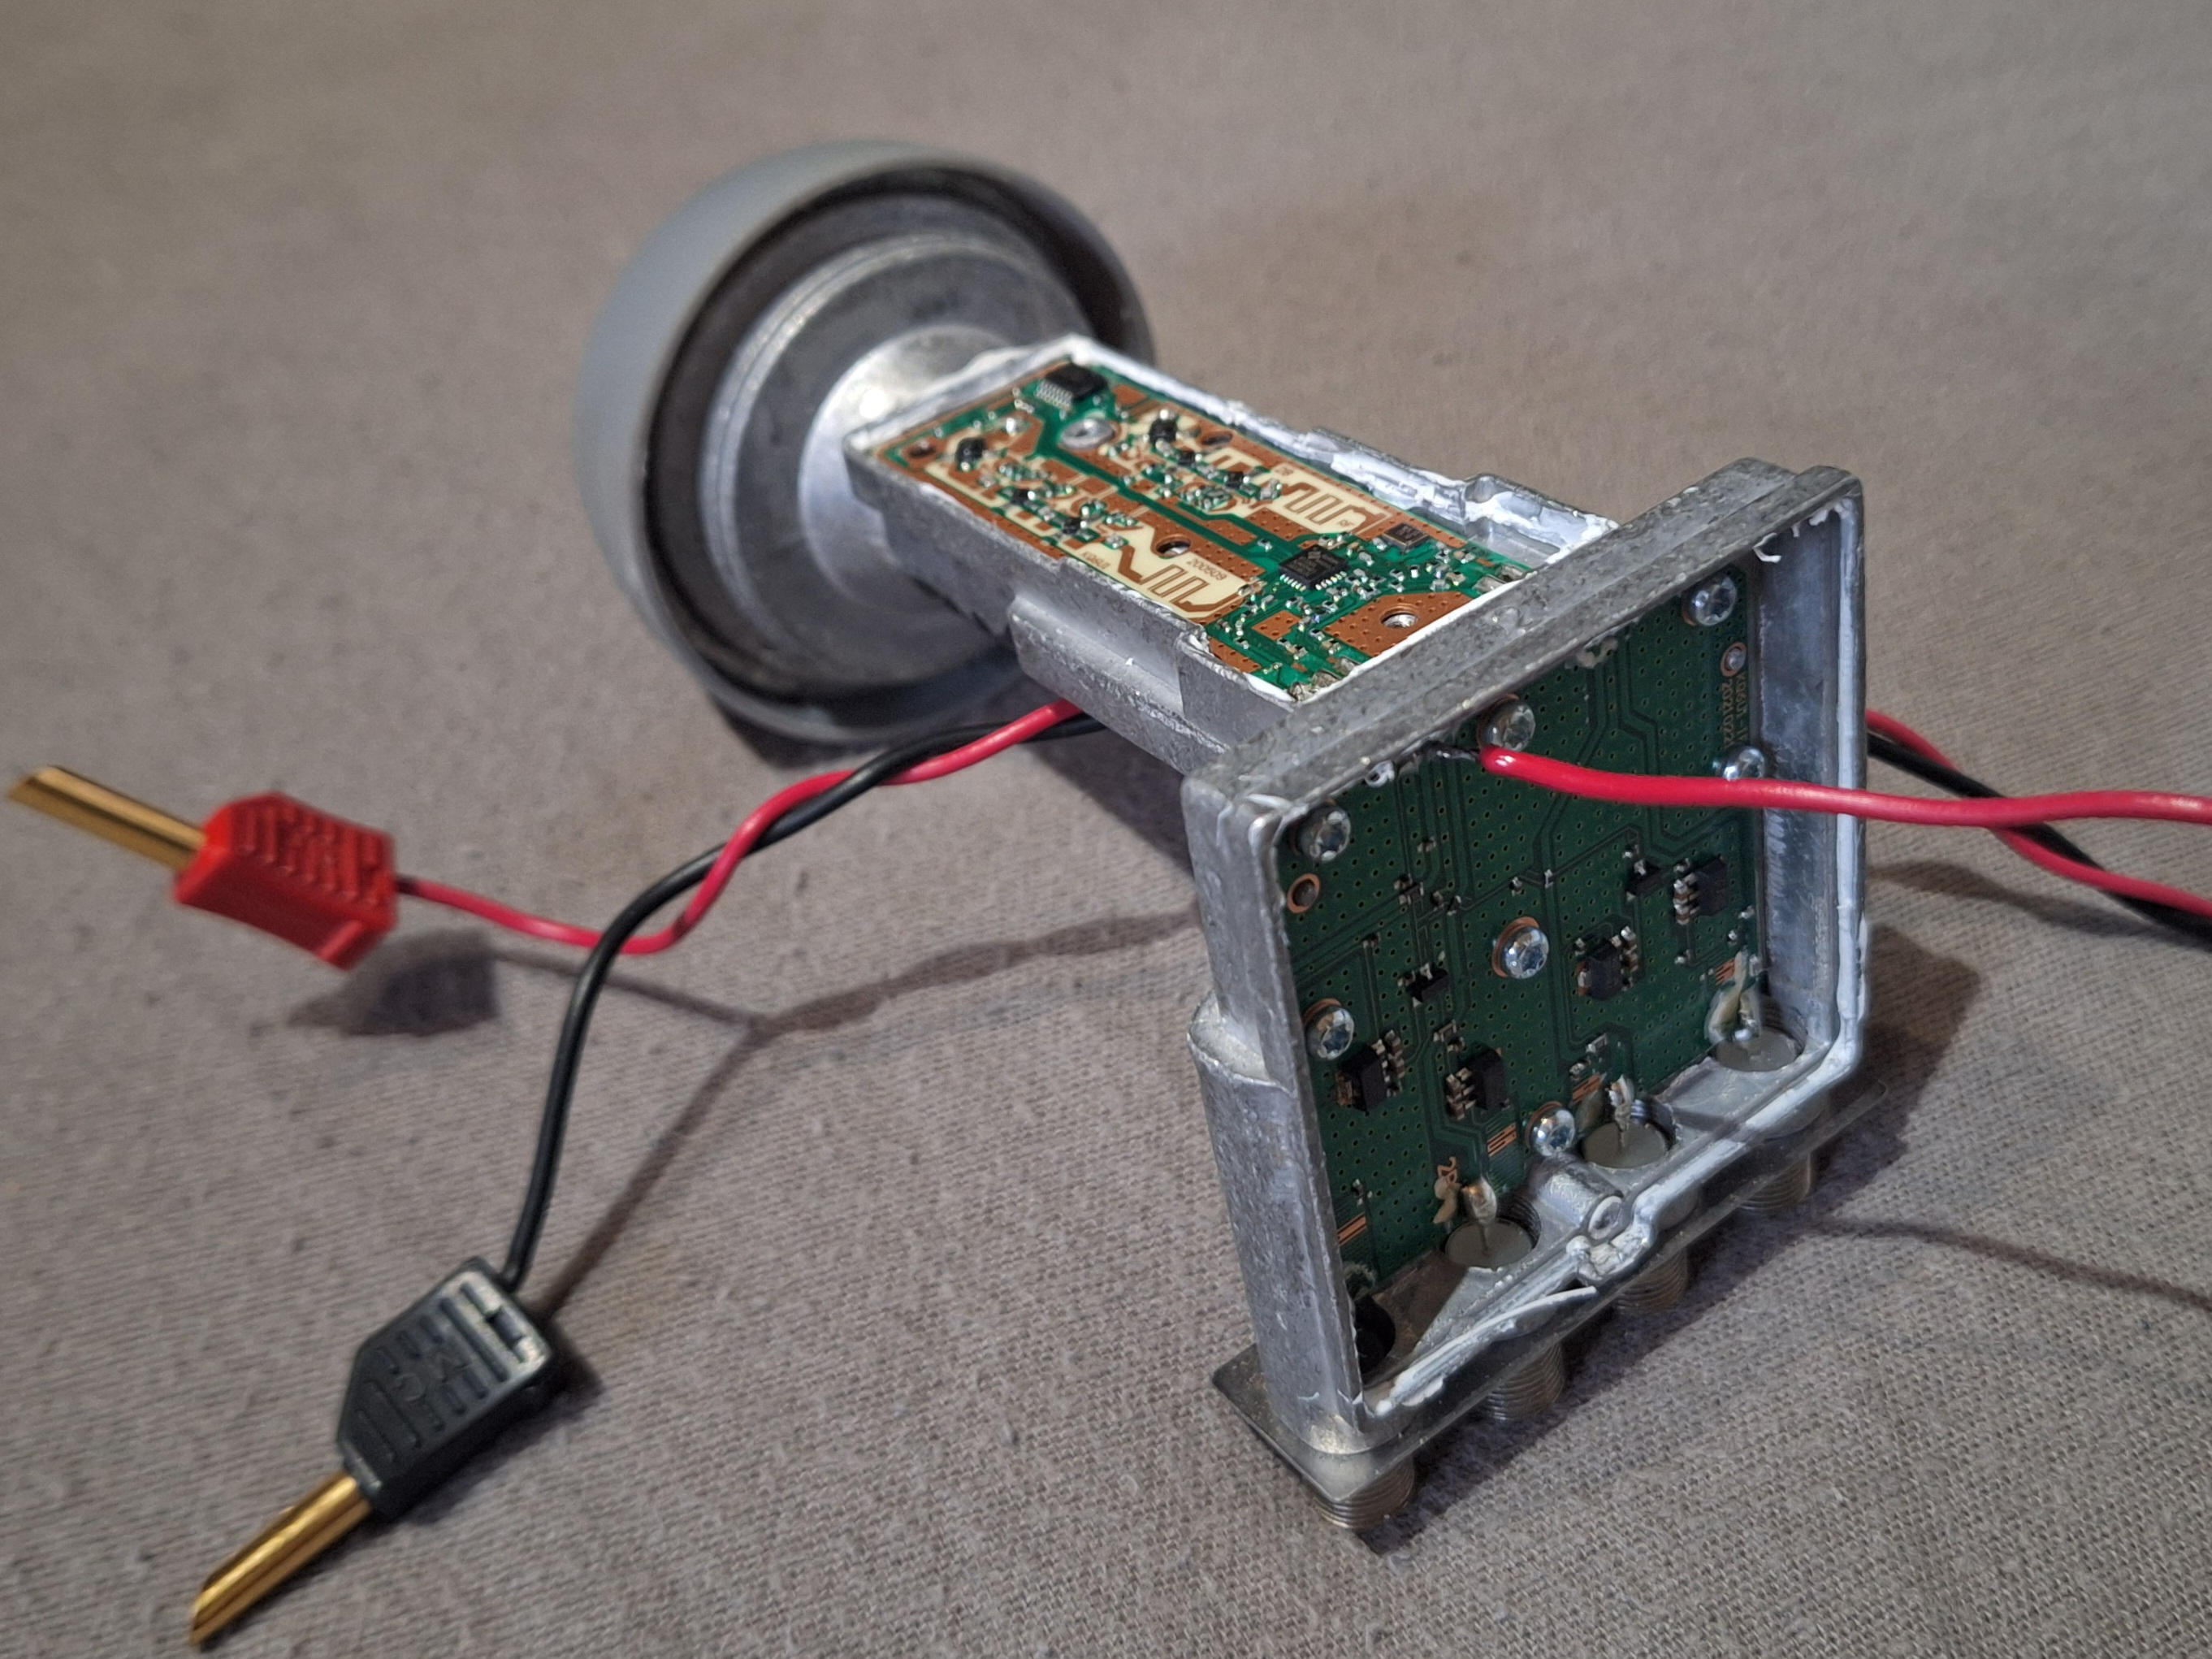
\includegraphics[width=0.8\textwidth]{./img/20250531_191954.jpg}
		\end{minipage}
	}
	\author{Sören Engelmann}
	
	
	
	\maketitle
	\newpage
	
	\section{Auseinanderbau}
	
	
	\section{Untersuchung der Platinen}
	
	\subsection{ZF-seitige Platine}
	
		
		\vspace{2ex}
		\begin{center}
			\begin{minipage}{0.7\textwidth}
				\centering
				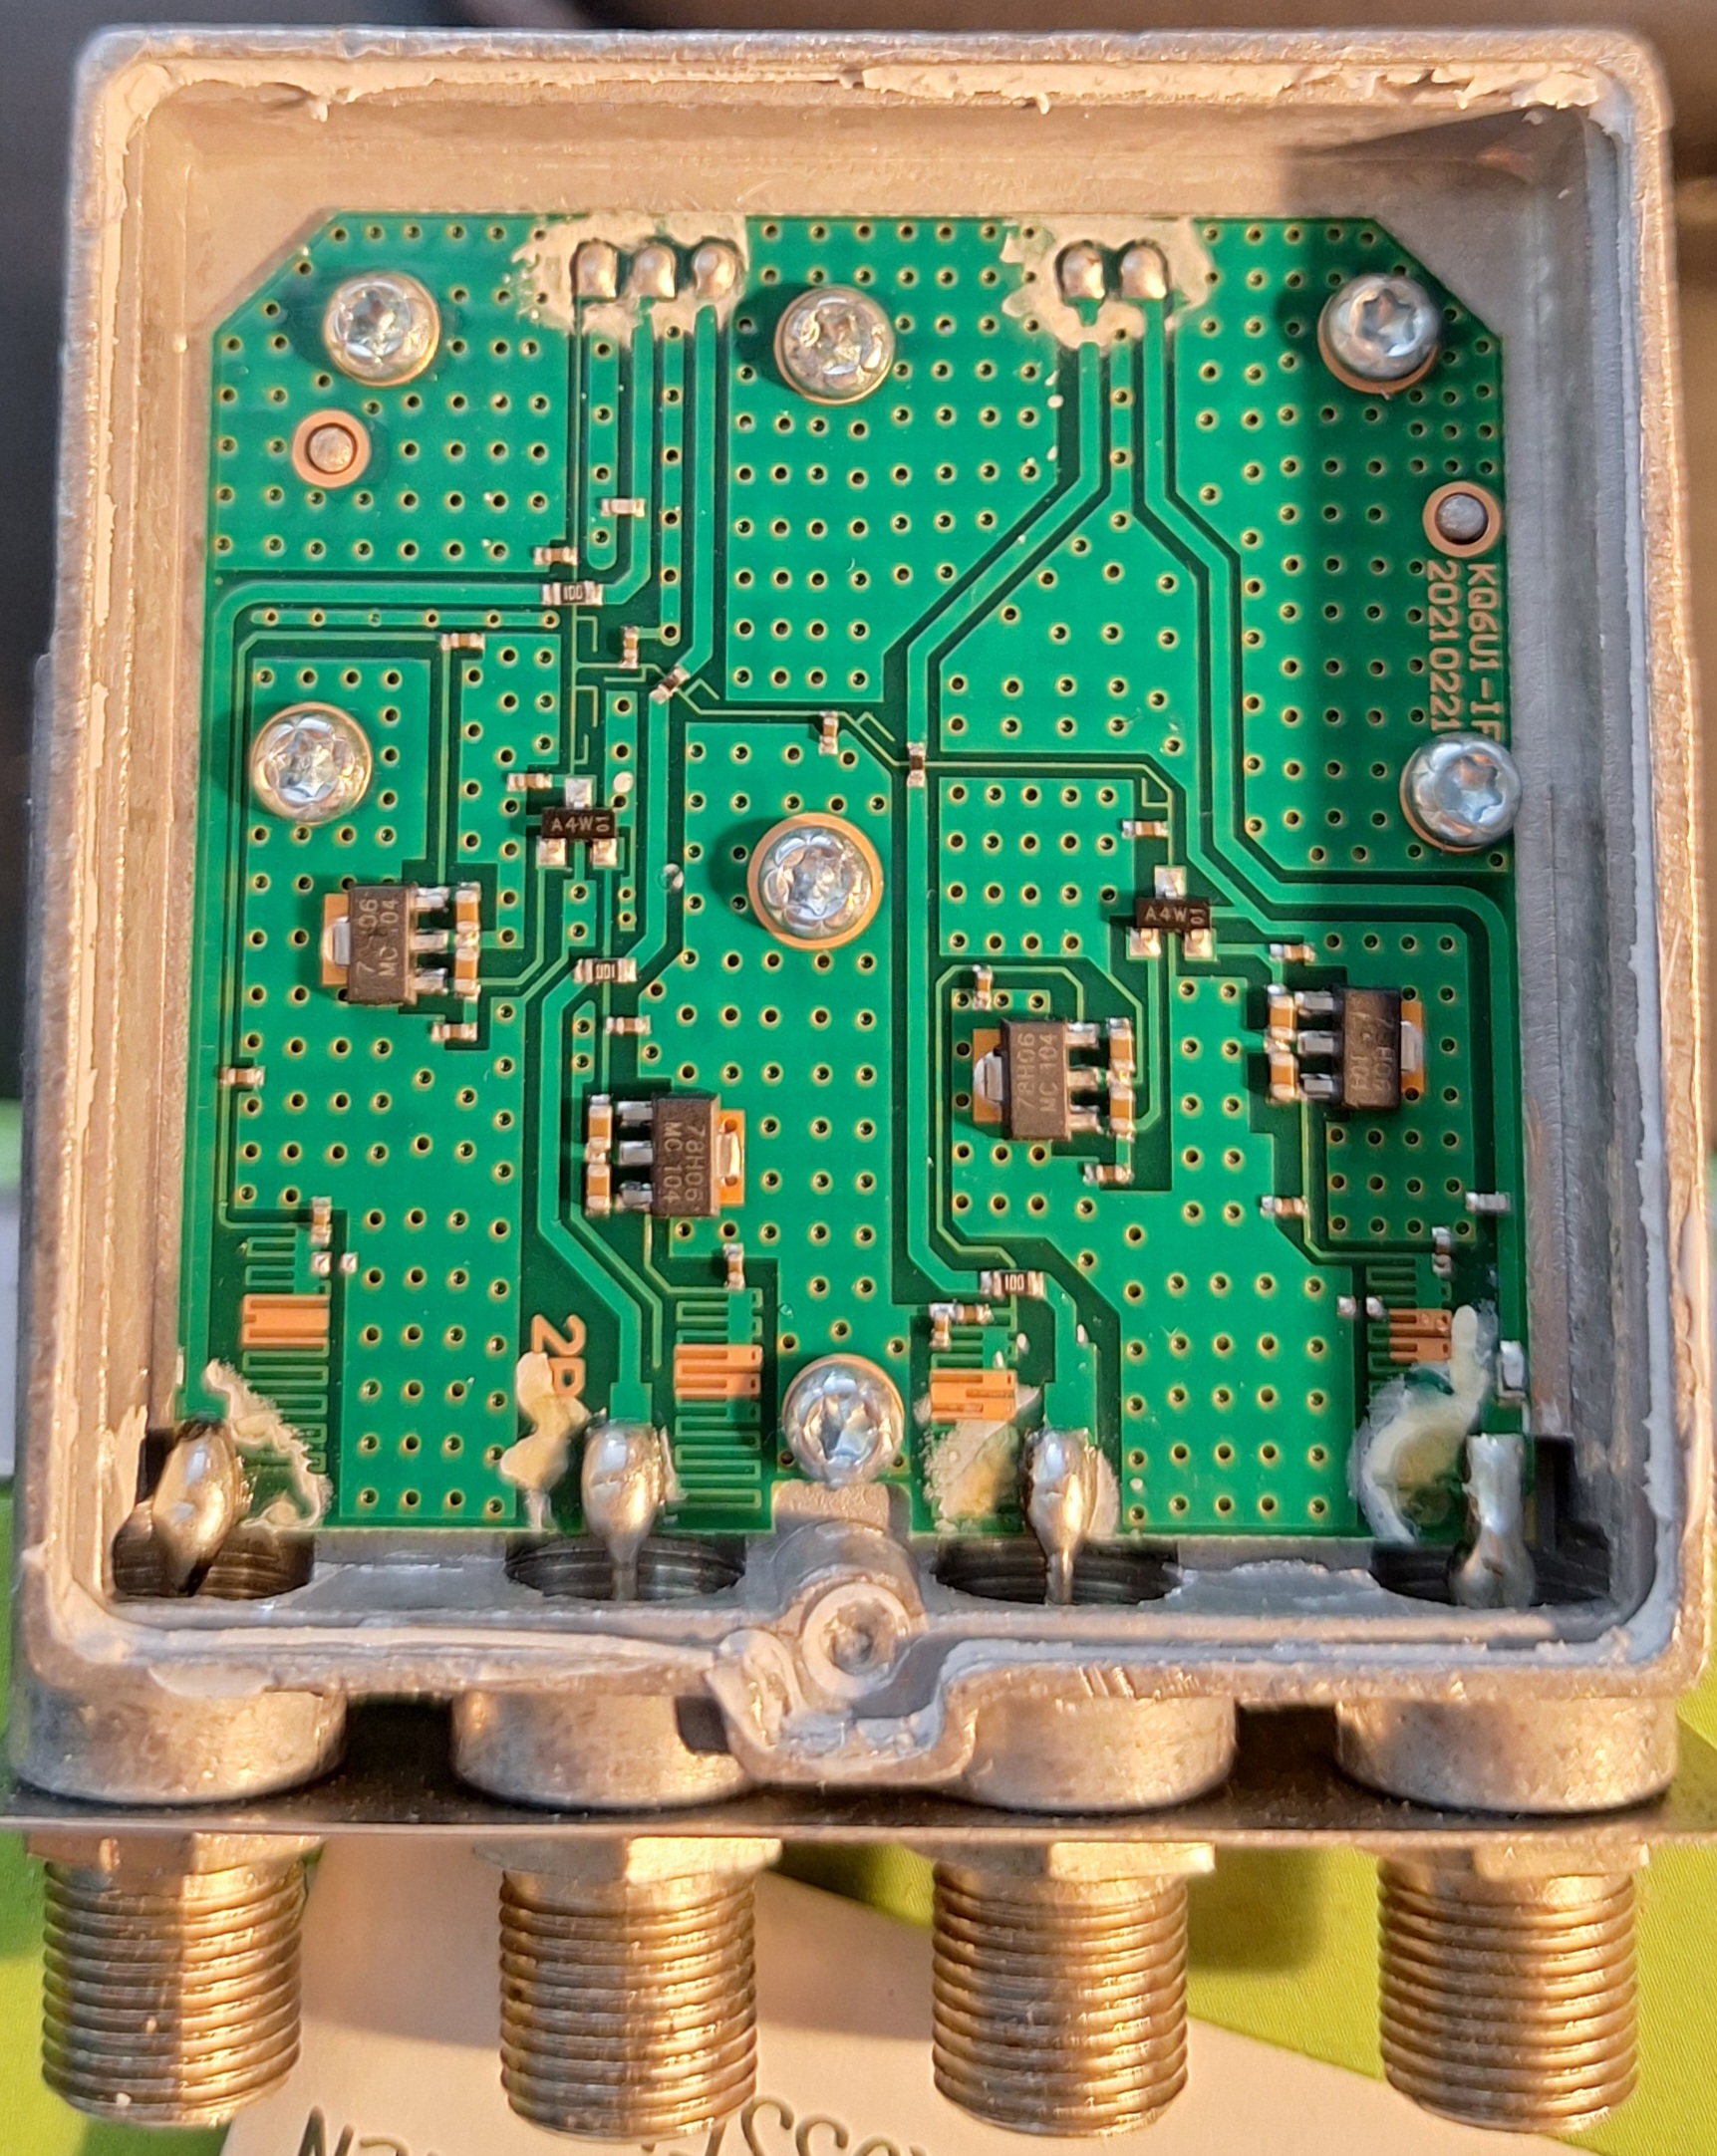
\includegraphics[height=\textwidth, angle=90]{./img/20250531_150218.jpg}
				\captionof{figure}{ZF-seitige Platine, Verbindungen zur HF-seitigen Platine links}
			\end{minipage}
		\end{center}
		\vspace{2ex}
		
		\noindent Unmittelbar an den vier Eingängen sind von den Haupt-Mikrostreifenleitungen abzweigende, gleich aufgebaute, mäanderförmige Mikrowellenstrukturen zu erkennen, die vermutlich einen Tiefpassfilter darstellen. Die Signalpfade wandern ohne großen Umweg durch je einen 10 Ohm Widerstand Richtung HF-seitige Platine.\\
		
	\subsubsection{78HC06 Linearregler}
		
		\noindent Die durch einen angeschlossenen Teilnehmer eingespeiste Spannung von 9.5 bis 19 V \parencite[siehe][]{Fuba417Manual} kann diesen passieren und findet jeweils ihren Weg zum Pin 3 eines ICs mit SOT-89-3 Gehäuse. Die aufgedruckten Markierungen sind 78HC06 und MC 104. Dieser Baustein wird als HT78H06ARDZ 6 V Linearregler von HTCSEMI identifiziert. Dieser ist bei LCSC zu finden \parencite[siehe][]{HT78H06ARDZ_LCSC}. Auf dem Vorschaubild bei LCSC ist ebenfalls das \glqq MC\grqq{} in der zweiten Reihe erkennbar. Bis auf eine Ziffer, vermutlich die Chargen- oder Fab-nummer, ist die Beschriftung gleich. Pin 3 ist laut Datenblatt \parencite[siehe][]{HT78H06ARDZ_Datasheet} Vin, also die Eingangsspannung. Aus dem Footprint auf der Leiterplatte kann auch eine Masseverbindung auf Pin 2 und Tab mit den sich im Datenblatt befindlichen Angaben abgeglichen werden. Zusätzlich sind zwei eng an den Anschlüssen platzierte MLCC-Kondensatoren zur Spannungsstabilisierung zu erkennen. Pin 1 ist demnach der Ausgang mit 6 V.\\
		
		\noindent \textit{Nebenbei sei noch angemerkt, dass Überschrift und Feature-Liste des Datenblatts, sowie die Angabe bei LCSC einen maximalen Ausgangsstrom von 0.3 A suggeriert, im Einleitungstext jedoch von 100 mA die Rede ist. Das kleine SOT-89-Gehäuse wäre sicherlich mit 100 mA eher zufriedener.}\\
		
		
	\subsubsection{BAV70 Diodenpacks}
		
		\noindent Die Ausgänge der vier Linearregler führen paarweise zu Pins 1 und 2 von ICs in einem SOT23-Gehäuse mit Markierung A4W 01. Durch eine Datenbank von SMD-Markierungen und den anschließenden Abgleich mit dem Datenblatt kann stark vermutet werden, dass es sich bei A4W um zwei integrierte Dioden mit gemeinsamer Kathode, Bezeichnung BAV70, vermutlich von Nexperia handelt \parencite[siehe][]{BAV70_Datasheet}. Diese sind Hochgeschwindigkeitsdioden mit einer reverse recovery time von 4 ns, jedoch vergleichweise hoher Vorwärtsspannung von 1 V bei 50 mA \glqq gepulst \grqq{}. Pins 1 und 2 stellen die Anoden dar. Folglich werden diese Diodenpacks vermutlich zur Vermeidung von Backfeeding in die Linearregler verwendet, wenn nicht alle vier Ausgänge des LNB in Benutzung sind.\\
		´
		\noindent Die Kathoden der beiden Diodenpacks treffen schließlich in einer gemeinsamen Leiterbahn aufeinander und laufen direkt zu den Verbindungen zur HF-seitigen Platine.\\
		
	\subsubsection{Beobachtungen zum Layout der Versorgungsspannungsleitung}
		
		\noindent An dieser Leiterbahn fallen zwei kuriose Dinge auf. Zum einen kreuzt diese nämlich auf dem Weg zur HF-seitigen Platine drei Mikrostreifenleitungen, da der Anschluss der Versorgungsspannung aus Sicht der ZF-seitigen Platine ganz links liegt. Auffällig ist, dass nicht etwa die Versorgungsspannung über 0 Ohm-Widerstände über diese hüpft, sondern dass die Mikrostreifenleitungen mit vermutlich kritischer Impedanz selbst aufgetrennt sind und über einen Widerstand als Brücke über die Versorgungsspannung hinweggeführt werden. Da diese wesentlich dünner ist, konnten als Brücken 0402 Bauformen verwendet werden, andersherum hätte man auf wesentlich größere Gehäuseformen zurückgreifen müssen.\\
		
		\noindent Außerdem fällt auf, dass an die Versorgungsspannung in regelmäßigen Abständen Stubs (Leerläufe) mit verschiedenen Längen angeschlossen sind. Vermutlich dienen diese als $\lambda/4$-Transformatoren und erzeugen bei kritischen Frequenzen auf der Versorgungsspannungsleitung einen Kurzschluss für eventuelle Störungen. Die Länge solch eines Arms beträgt etwa 3 mm ($\rightarrow\lambda/4$), was bei Mikrostreifenleitungen auf FR4-Substrat ($\epsilon_{r\text{,eff}}\approx4$) laut Online-Rechner in einer Frequenz von 12.5 GHz, also ungefähr der Eingangsfrequenz des LNBs resultiert. Vermutlich zeigten sich dort während der Entwicklung Probleme durch Einkopplungen in die Versorgungsspannung, vielleicht sogar durch Diodenpacks und Linearregler bis in die Ausgänge.
		
	\subsection{HF-seitige Platine}
	
	
	\vspace{2ex}
	\begin{center}
		\begin{minipage}{0.9\textwidth}
			\centering
			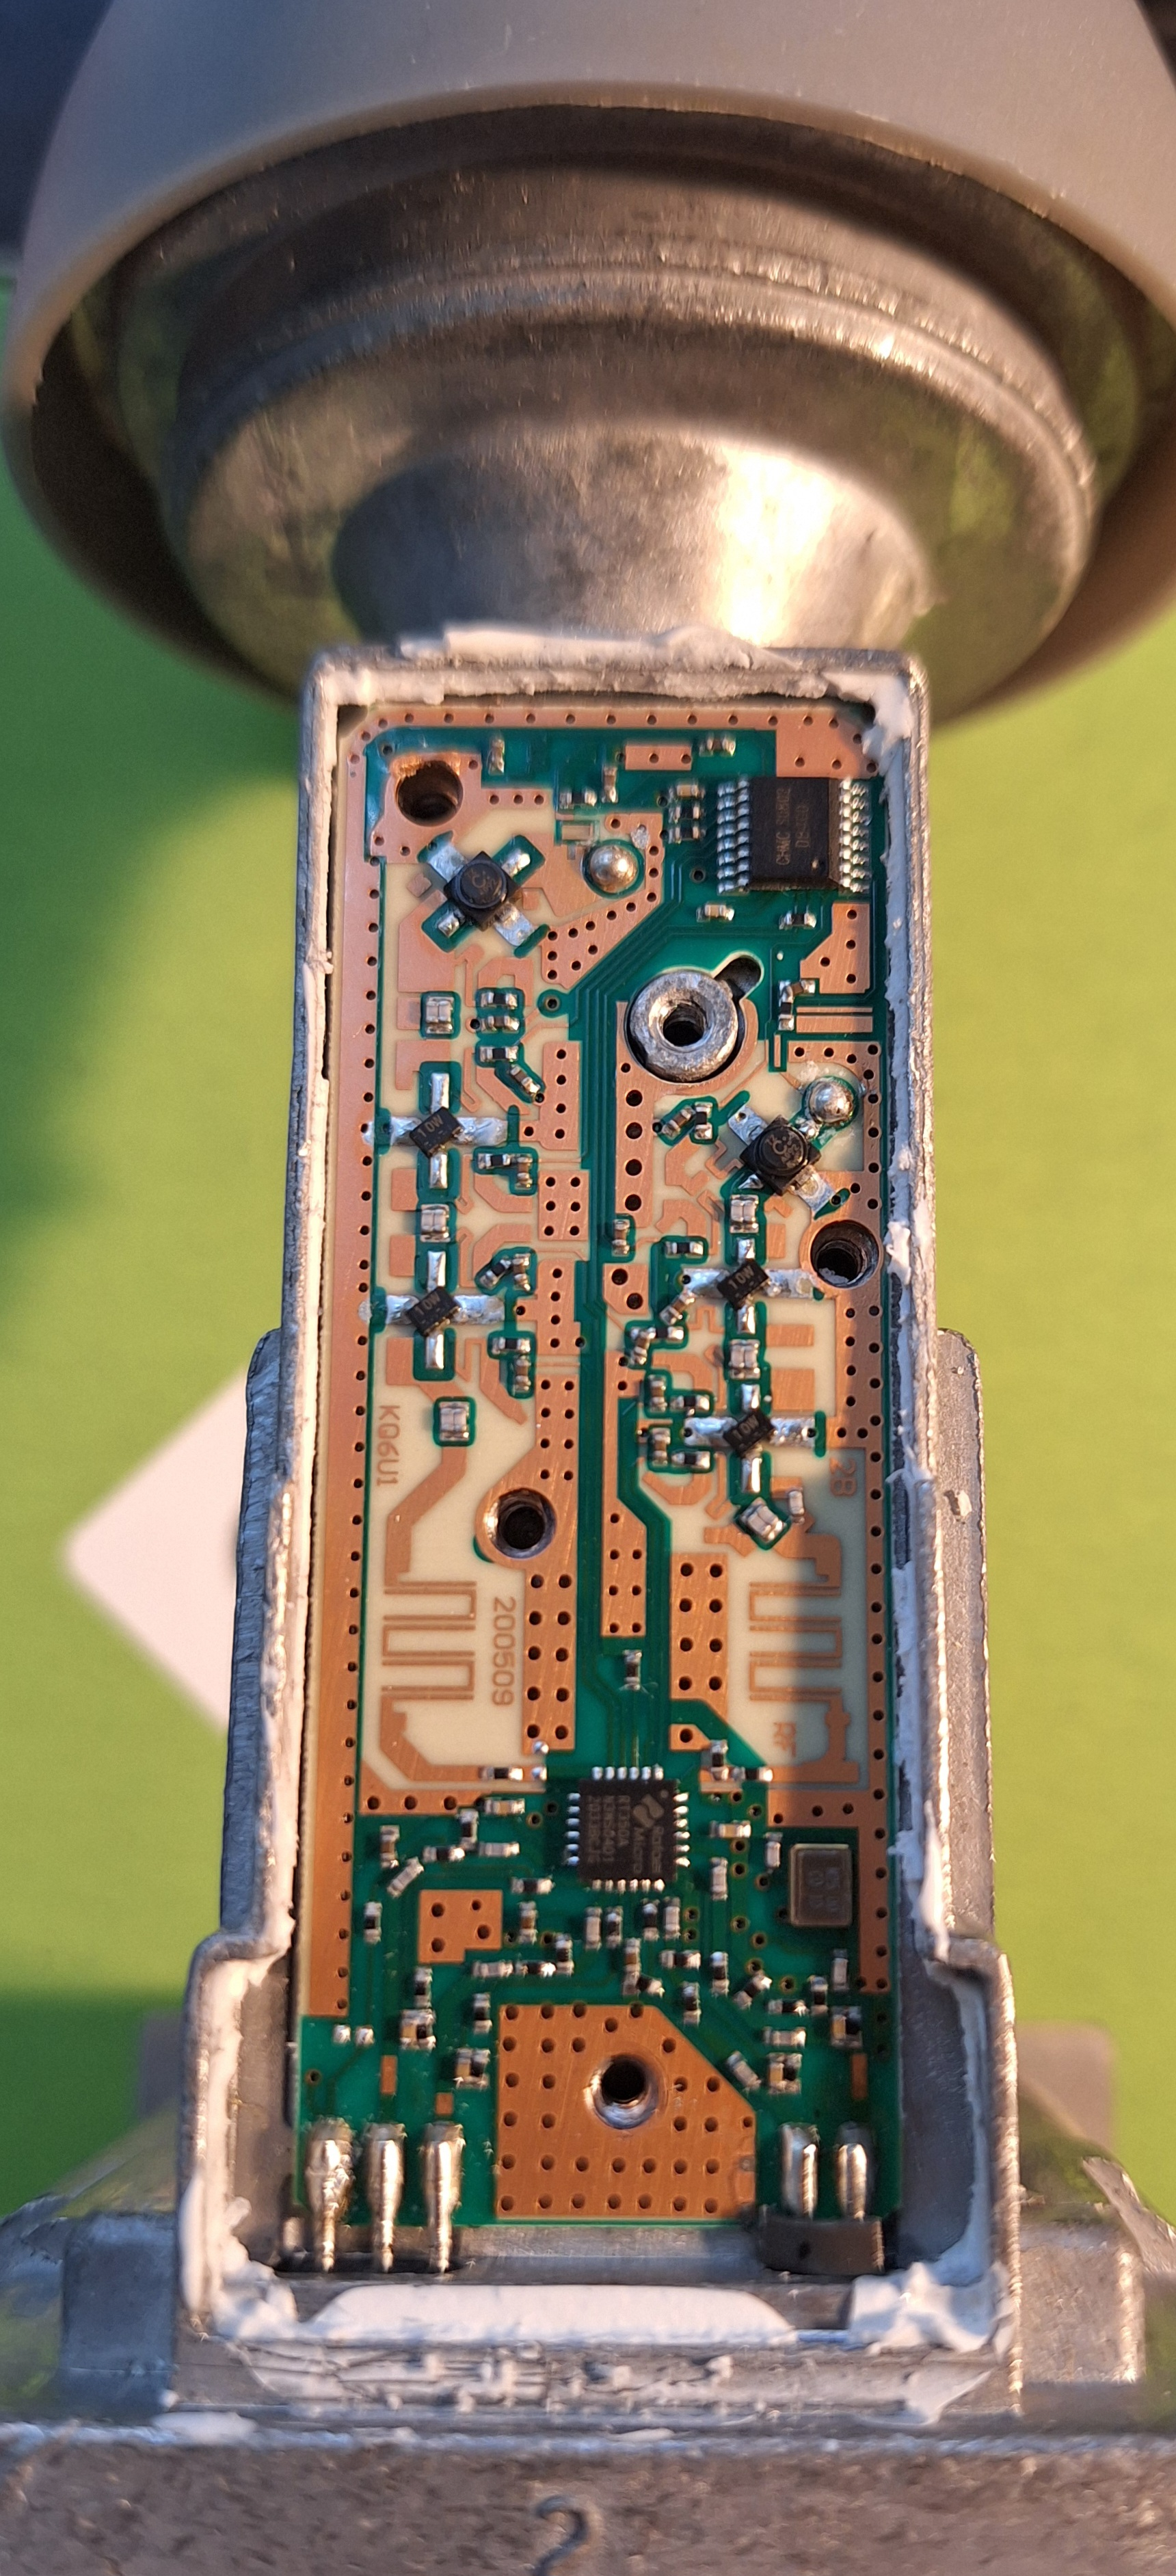
\includegraphics[height=\textwidth, angle=90]{./img/20250531_150332.jpg}
			\captionof{figure}{HF-seitige Platine, Verbindungen zur ZF-seitigen Platine rechts}
		\end{minipage}
	\end{center}
	\vspace{2ex}
	
	
	\subsubsection{25 MHz Quarz}
	
		\noindent Unter Suche der Markierungen \glqq M25.00 CQ 1D\grqq{} des Quarzes und Abgleich des Gehäuses kann vermutet werden, dass es sich um einen 25 MHz-Quarz von Quantek aus der QC5A Serie, genauer den QC5A25.0000F12B33M handelt. Pins 2 und 4 sind augenscheinlich mit Masse verbunden, was sich mit der Pinbelegung des Datenblatts deckt. Aufgrund der kleinen SMD-Pads des verwendeten Footprints lässt sich dies jedoch nicht vollends überprüfen. Zu diesem Zeitpunkt der Untersuchungen ohne endgültigen Plan für einen Umbau wird auf ein Entlöten dieses Quarzes vorerst verzichtet.
		
	\subsubsection{Downconverter Rafael Micro RT350A}
		
		\noindent Zu Beginn sei gesagt, dass der spezifische Downconverter RT350A von Rafael Micro nicht dokumentiert ist. Dieser ist auch bei keinem mir bekannten Distributor erhältlich. Alles nachfolgende wird durch Transfer von verwandten Bausteinen und eigenem Reverse Engineering zusammengetragen.\\
		
		\noindent Auf der Homepage von Rafael Micro \cite{RafaelMicro} finden sich diverse Downconverter speziell für den Einsatz für den Satellitenempfang, diese sind dort tabellarisch aufgeführt. Dort tauchen auch Downconverter ICs mit ähnlicher Teilenummer auf:\\
		
		
		\begin{minipage}{\textwidth}
			{\scriptsize
				\begin{tabular}{llllll}
					Part No & Ku-band LNB RF Downconverter & Control & Input Range (GHz) & LO (GHz) & Vcc (V)\\
					$\vdots$ & $\vdots$ & $\vdots$ & $\vdots$ & $\vdots$ & $\vdots$\\
					RT342M & Quad & 13 / 18VDC & 11.70 \~ 12.75 & 10.75 & 5.0\\
					RT343M & Quad & 13 / 18VDC & 12.25 \~ 12.75 & 11.30 & 5.0\\
					RT346M & Quattro Universal & - & 11.70 \~ 12.75 & 10.75 & 3.3\\
					RT348M & Quattro Universal & - & 11.70 \~ 12.75 & 10.75 & 5.0\\
					$\vdots$ & $\vdots$ & $\vdots$ & $\vdots$ & $\vdots$ & $\vdots$
				\end{tabular}
			}\captionof{table}{Auszug aus dem Produktangebot von Rafael Micro.\label{tab:RafaelMicro_Downconverters}}
		\end{minipage}
		
		
		\noindent Da es sich hier beim Fuba DEK 417 um einen Quad LNB handelt, wird davon ausgegangen, dass der hier verbaute IC RT350A mit dem RT342M, beziehungsweise em RT343M verwandt ist. Als Betriebsspannung ist hier 5 Volt angegeben. Durch Untersuchung der ZF-seitigen Platine \ref{label} wurde dort eine entsprechende Versorgung von etwa 5 Volt identifiziert.\\
		
		\noindent Der vorliegende LNB ist jedoch im Unterschied zu den genannten Artverwandten mit Eingangsfrequenzbereichen von 10.7 GHz bis 11.7 GHz, beziehungsweise 11.7 GHz bis 12.75 GHz. Somit muss der RT350A ein Hybrid aus den in Tabelle \ref{tab:RafaelMicro_Downconverters} aufgeführten Bausteinen sein.\\
		
		\vspace{2ex}
		\begin{center}
			\begin{minipage}{0.9\textwidth}
				\centering
				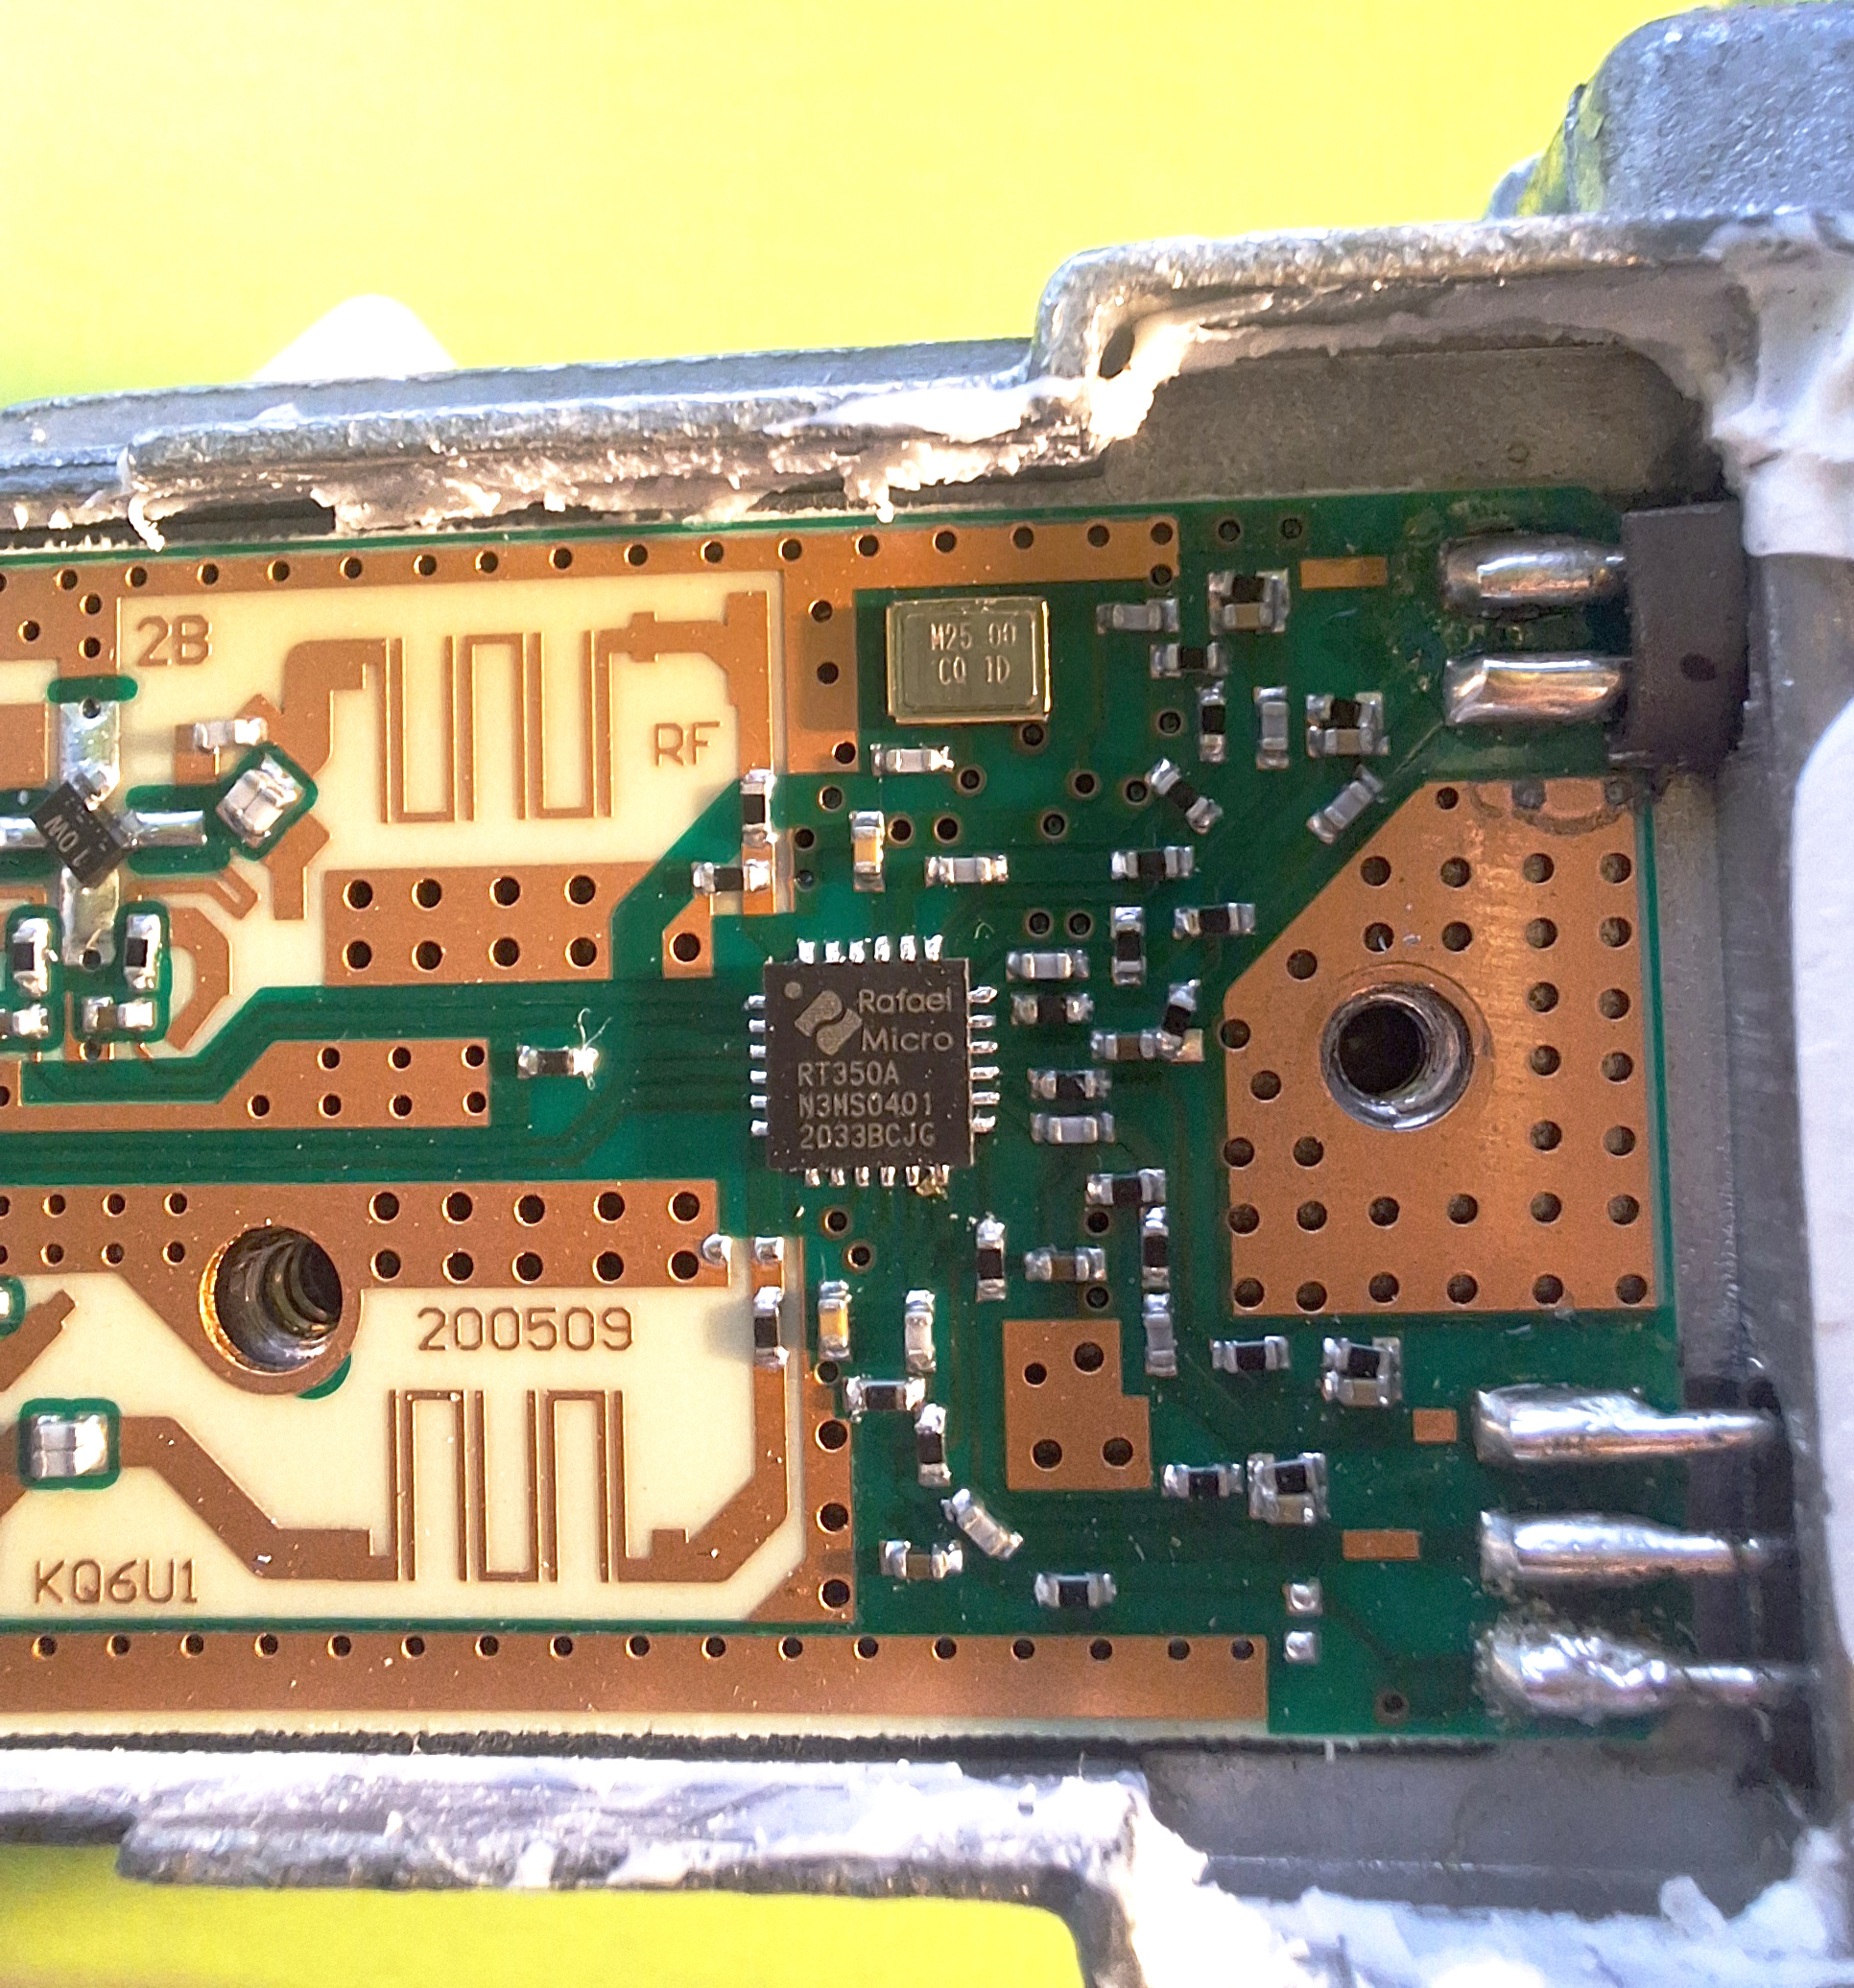
\includegraphics[width=\textwidth, trim=0 2cm 0 4cm, clip]{./img/20250531_150421.jpg}
				\captionof{figure}{Detailansicht von RT350A IC und Verbindungen}
			\end{minipage}
		\end{center}
		\vspace{2ex}
		
		
		\noindent Der RT350A sitzt in einem TQFN-24 Gehäuse mit exponiertem Thermal Pad. Der Pin für die 5V-Versorgungsspannung kann ermittelt werden, indem die Versorgungsschiene ab der Durchführung zum ZF-seitigen Teil bis hin zum IC verfolgt wird. Diese endet an Pin 16. Eine mit Masse verbundene, relativ breite Leitung führt augenscheinlich zum Thermal Pad, was sich unter aus dem Gesichtspunkt erklären lässt, dass außer Pin 3 über einen 0 Ohm-Jumper kein sonstiger Pin mit Masse verbunden ist.\\
		
		\noindent Pins 1, 2 und 4, 5 führen jeweils zu verschiedenen Abgriffen an der Kette von je drei LNA-Stufen pro Polarisationspfad. Eventuell stellen diese eine Art AGC dar und können LNAs aktivieren oder deaktivieren, dies ist lediglich eine Vermutung. In Pins 24 und 6 enden die Pfade ausgehend von den jeweiligen Antennen für die beiden Polarisationen. Mutmaßlich keine Verbindung haben Pins 7, 8, 22, 23. Die vier Ausgänge in Richtung ZF-seitige Platine enden nach Anpassungs- oder Filternetzwerken in Pins 12, 14, 18 und 20. Von Wichtigkeit sind noch die beiden Pins 9 und 10, an die der Quarz angeschlossen ist. Sonstige Verbindungen lassen sich ohne größeren Aufwand so nicht nachvollziehen.
	
	
	\begin{minipage}{\textwidth}
		\centering
		\begin{circuitikz}
			\ctikzset{multipoles/font={\color{red}\tiny}}
			\draw (0,0) node[qfpchip,
			num pins=24,
			external pad fraction=6](C){}; %RT350A
			
			\draw (C.pin 1) node[anchor=east]{POL1\_SENSE1?};
			\draw (C.pin 2) node[anchor=east]{POL1\_SENSE2?};
			\draw (C.pin 3) node[anchor=east]{GND};
			\draw (C.pin 4) node[anchor=east]{POL2\_SENSE2?};
			\draw (C.pin 5) node[anchor=east]{POL2\_SENSE1?};
			\draw (C.pin 6) node[anchor=east]{POL2\_FEED};
			
			\draw (C.pin 7) node[anchor=east,rotate=90]{NC};
			\draw (C.pin 8) node[anchor=east,rotate=90]{NC};
			\draw (C.pin 9) node[anchor=east,rotate=90]{XTAL1};
			\draw (C.pin 10) node[anchor=east,rotate=90]{XTAL2};
			\draw (C.pin 11) node[anchor=east,rotate=90]{?};
			\draw (C.pin 12) node[anchor=east,rotate=90]{OUT1};
			
			\draw (C.pin 13) node[anchor=west]{?};
			\draw (C.pin 14) node[anchor=west]{OUT2};
			\draw (C.pin 15) node[anchor=west]{?};
			\draw (C.pin 16) node[anchor=west]{VCC 5V};
			\draw (C.pin 17) node[anchor=west]{?};
			\draw (C.pin 18) node[anchor=west]{OUT3};
			
			\draw (C.pin 19) node[anchor=west,rotate=90]{?};
			\draw (C.pin 20) node[anchor=west,rotate=90]{OUT4};
			\draw (C.pin 21) node[anchor=west,rotate=90]{?};
			\draw (C.pin 22) node[anchor=west,rotate=90]{NC};
			\draw (C.pin 23) node[anchor=west,rotate=90]{NC};
			\draw (C.pin 24) node[anchor=west,rotate=90]{POL1\_FEED};
			
			\draw (C) node[shape=rectangle, minimum width=20mm, minimum height=20mm,draw=black]{GND};
			
			%\draw (C.pin 1) -- ++(-0.5,0) to[R] ++(0,-2) node[ground]{};
		\end{circuitikz}
		\captionof{figure}{Partielles Pinout von Rafael Micro RT350A.\label{fig:RafaelMicro_Pinout}}
	\end{minipage}\vspace{2ex}
	
	\noindent Bisher ungeklärt ist, welcher der beiden Pins für den Quarz Eingang, beziehungsweise Ausgang des Inverters oder Taktgenerators ist. %Als einfachen Test werden die beiden Eingangswiderstände der Pins ohne anliegende Versorgungsspannung mit dem Widerstandsmodus des Multimeters gegen Masse gemessen. Pin 9 hat nach Masse hin etwa 40.2 k$\Omega$, Pin 10 etwa 16 k$\Omega$ (rot auf Masse), beziehungsweise 17.8 k$\Omega$ (schwarz auf Masse). Die Impedanzen unterscheiden sich nicht in der erhofften Größenordnung, somit kann nicht zweifelsfrei auf eine niederohmige Ausgangsstufe und hochohmige Eingangsstufe geschlossen werden.\\
	%\noindent Da diese mittelalterliche Methode nicht funktioniert hat, wird 
	Dazu wird der RT350A nun in Betrieb genommen. Über die Kathode einer der beiden Diodenpacks sowie das Alu-Gehäuse als Masse wird eine Versorgungsspannung von 5 V eingespeist. Bei einer mit dem verwendeten Labornetzgerät QJE3005E~III nicht detektierbaren Stromaufnahme läuft das IC an. Mit dem x10-Tastkopf des Oszilloskops (SIGLENT~SDS~1102CNL) sind deutliche 25 MHz-Signale an beiden Pins sichtbar. Pin 9 zeigt einen sinusförmigen Verlauf mit ca. 896 mVpp und schwingt augenscheinlich frei, während Pin 10 einen stark verzerrten Sinusverlauf mit etwa 696 mVpp aufweist. Aufgrund der Verzerrung wird darauf geschlossen, dass Pin 10 den Ausgang des Inverters und Pin 9 den entsprechenden Eingang darstellt, obwohl bei diesem eine niedrigere Spitze-zu-Spitze-Spannung messbar ist.
	
	\vspace{2ex}
	\begin{minipage}{0.9\textwidth}
		\centering
		\begin{tabular}{rl}
			
			\begin{minipage}{0.5\textwidth}
				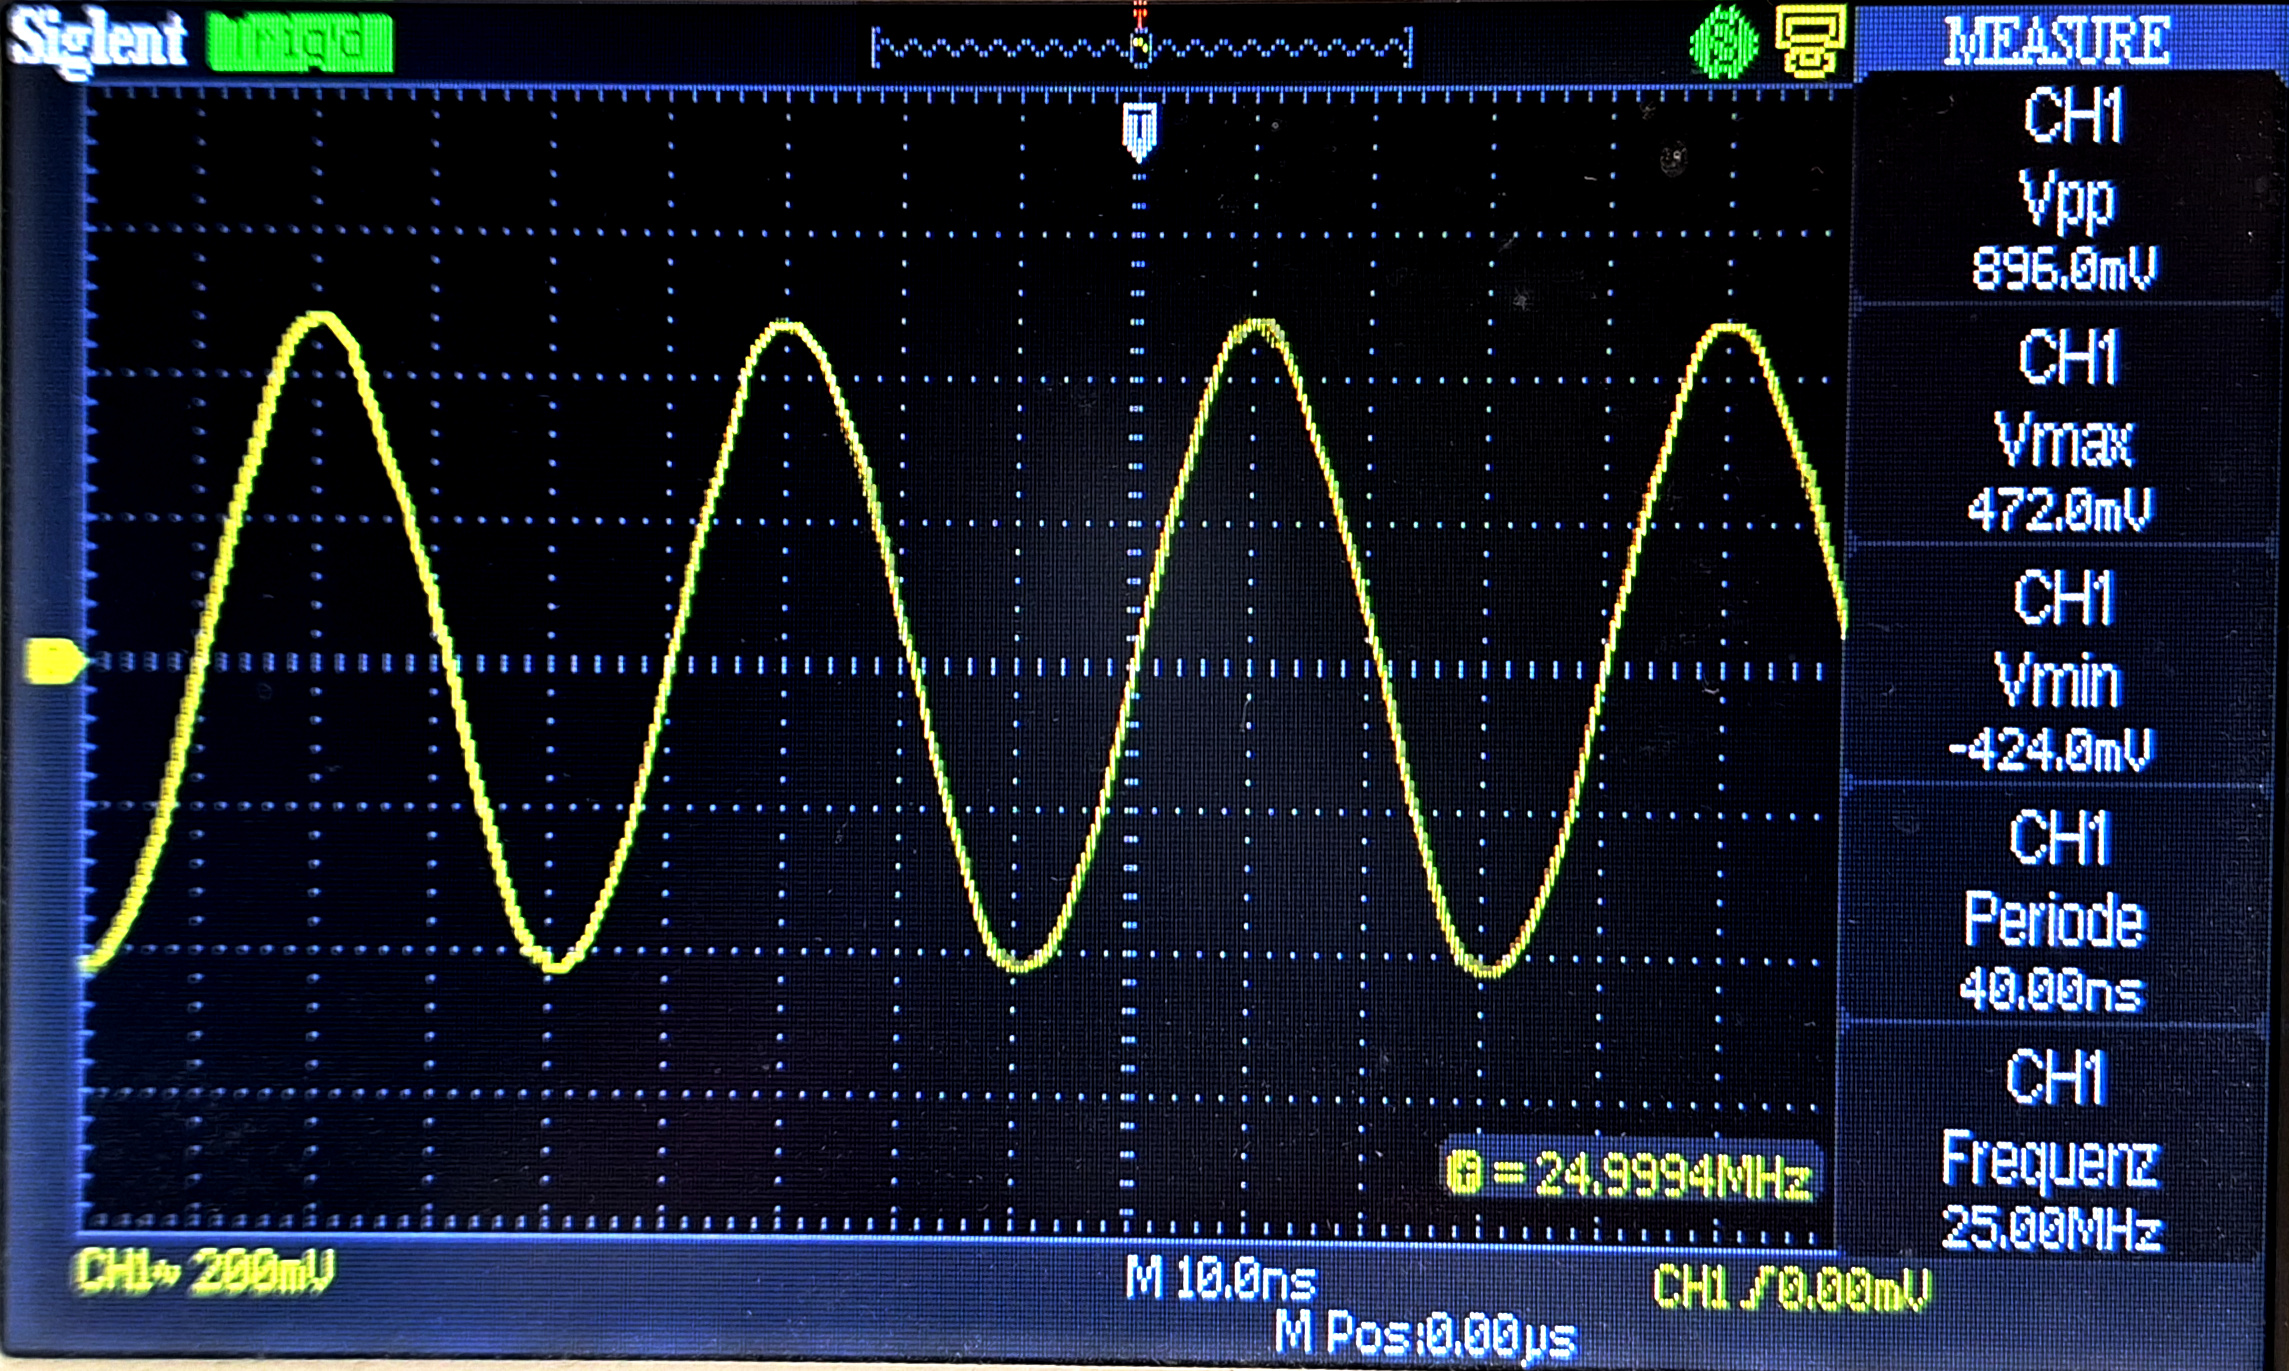
\includegraphics[width=\textwidth]{./img/Pin 9.jpg}
				\captionof{figure}{Pin 9, AC Kopplung}
			\end{minipage}
			&
			\begin{minipage}{0.5\textwidth}
				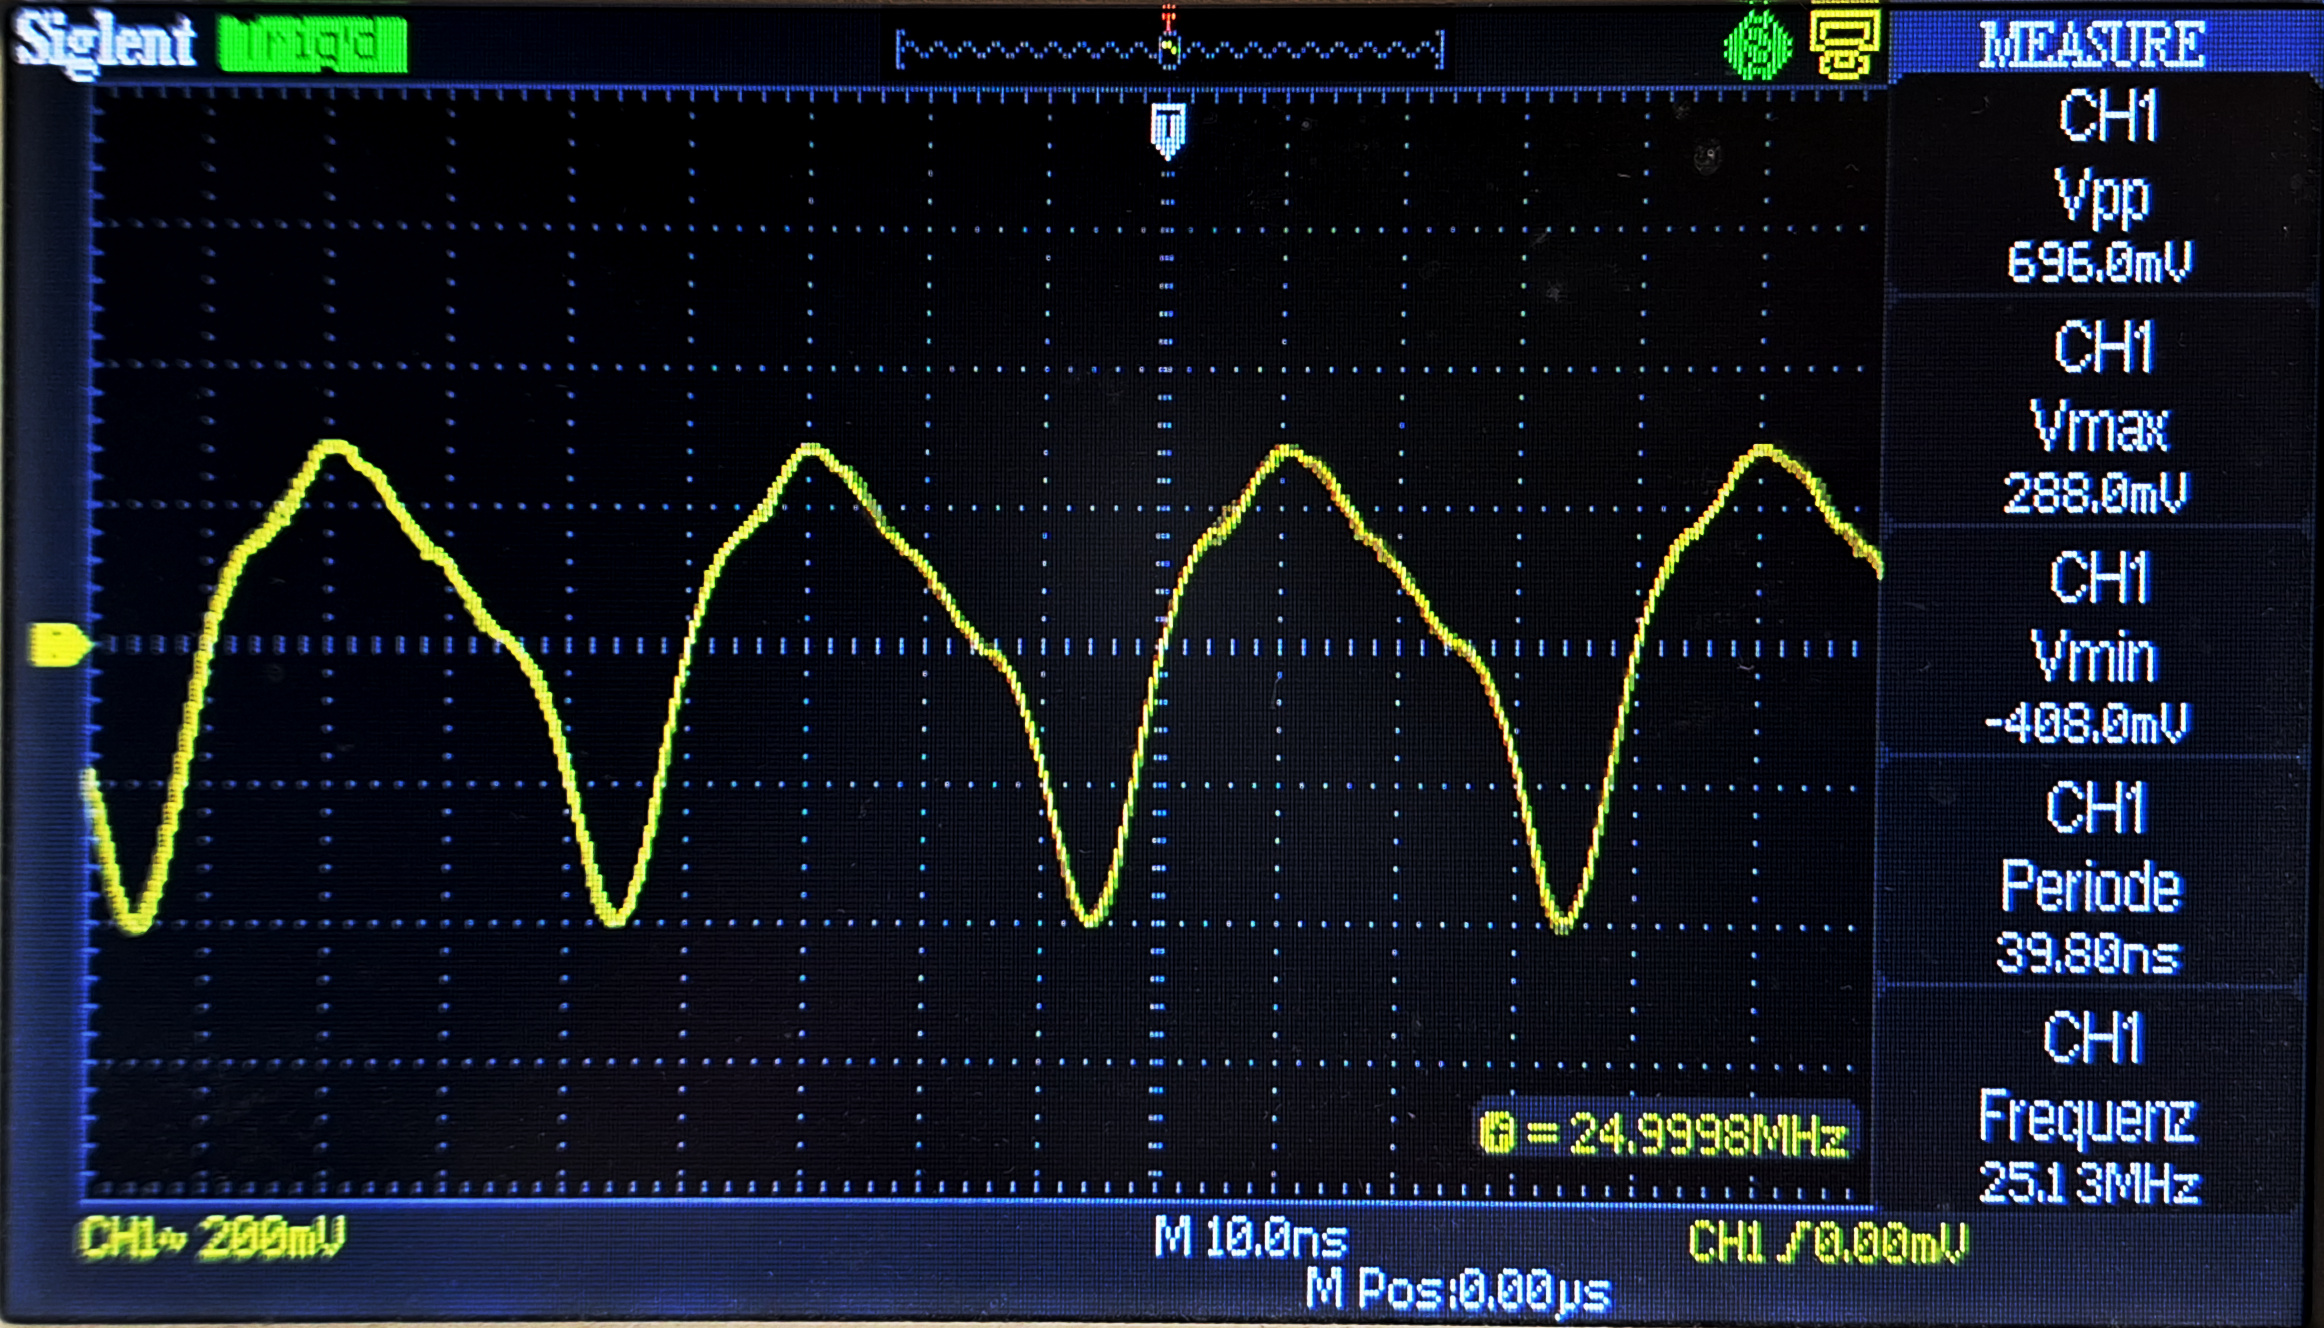
\includegraphics[width=\textwidth]{./img/Pin 10.jpg}
				\captionof{figure}{Pin 10, AC Kopplung}
			\end{minipage}
		\end{tabular}
	\end{minipage}
	\vspace{2ex}
	
	
	\section{Modifikation der Spannungsversorgung}
	
	
	\section{Modifikation des 25 MHz Takteingangs}
	
	
	\printbibliography
\end{document}